\documentclass[10pt,a4paper]{article}
\usepackage[utf8]{inputenc}
\usepackage[T1]{fontenc}
\usepackage{amsmath}
\usepackage{amssymb}
\usepackage{graphicx}
\usepackage[english]{babel}
\usepackage{booktabs}
\usepackage{array}
\usepackage{placeins}

\usepackage{url}
\usepackage{hyperref}
\usepackage{listings}
\usepackage{textcomp}
\usepackage{accsupp}
\usepackage{attachfile}

% color def
\usepackage{color}
\definecolor{darkred}{rgb}{0.6,0.0,0.0}
\definecolor{darkgreen}{rgb}{0,0.50,0}
\definecolor{lightblue}{rgb}{0.0,0.42,0.91}
\definecolor{orange}{rgb}{0.99,0.48,0.13}
\definecolor{grass}{rgb}{0.18,0.80,0.18}
\definecolor{pink}{rgb}{0.97,0.15,0.45}

% listings
\usepackage{listings}

% General Setting of listings
\lstset{
	language=Python,
	tabsize=4,
	aboveskip=1em,
	breaklines=true,
	abovecaptionskip=-6pt,
	captionpos=b,
	escapeinside={\%*}{*)},
	frame=single,
	numbers=left,
	numbersep=8pt,
	numberstyle=\tiny,
	morekeywords=[1]{,as,assert,nonlocal,with,yield,self,True,False,None,} % Python builtin
	morekeywords=[2]{,__init__,__add__,__mul__,__div__,__sub__,__call__,__getitem__,__setitem__,__eq__,__ne__,__nonzero__,__rmul__,__radd__,__repr__,__str__,__get__,__truediv__,__pow__,__name__,__future__,__all__,}, % magic methods
	morekeywords=[3]{,object,type,isinstance,copy,deepcopy,zip,enumerate,reversed,list,set,len,dict,tuple,range,xrange,append,execfile,real,imag,reduce,str,repr,}, % common functions
	morekeywords=[4]{,Exception,NameError,IndexError,SyntaxError,TypeError,ValueError,OverflowError,ZeroDivisionError,}, % errors
	morekeywords=[5]{,ode,fsolve,sqrt,exp,sin,cos,arctan,arctan2,arccos,pi, array,norm,solve,dot,arange,isscalar,max,sum,flatten,shape,reshape,find,any,all,abs,plot,linspace,legend,quad,polyval,polyfit,hstack,concatenate,vstack,column_stack,empty,zeros,ones,rand,vander,grid,pcolor,eig,eigs,eigvals,svd,qr,tan,det,logspace,roll,min,mean,cumsum,cumprod,diff,vectorize,lstsq,cla,eye,xlabel,ylabel,squeeze,}, % numpy / math
	deletekeywords=[2]{next,set},
	deletekeywords=[3]{next,set},
	basicstyle=\ttfamily,
	backgroundcolor=\color{white},
	commentstyle=\color{darkgreen}\slshape,
	keywordstyle=\color{blue}\bfseries\itshape,
	keywordstyle=[2]\color{blue}\bfseries,
	keywordstyle=[3]\color{grass},
	keywordstyle=[4]\color{red},
	keywordstyle=[5]\color{orange},
	stringstyle=\color{darkred},
	emphstyle=\color{pink}\underbar,
	morestring=[d]{"},
	showstringspaces=false,
	upquote=true,
}

\usepackage{tikz}
\usetikzlibrary{calc,shapes.multipart,chains,arrows,positioning}

\makeatletter
\lst@RequireAspects{writefile}

% Use \attachfile command to add listing content as paperclip.
\lstnewenvironment{attachedlisting}[1][]{%
	\lst@BeginAlsoWriteFile{#1.txt}%
}
{%
	\lst@EndWriteFile
	\marginpar{\attachfile[appearance=false,icon=Paperclip,mimetype=text/tex]{#1.txt}}
}

% Use accsupp package to add listing content as copyable text.
\lstnewenvironment{copyablelisting}{%
	\lst@BeginAlsoWriteFile{\jobname.txt}%
}
{%
	\lst@EndWriteFile
	\let\verbatim@processline\add@lstline
	\global\let\lstfile\empty
	\verbatiminput{\jobname.txt}%
	\marginpar{(\BeginAccSupp{method=escape,ActualText={\lstfile}}\PaperPortrait\EndAccSupp{})}
}
\def\add@lstline
{\xdef\lstfile{\unexpanded\expandafter{\lstfile}\the\verbatim@line\string^^J}}
\makeatother

\tikzset{
	squarecross/.style={
		draw, rectangle,minimum size=18pt, fill=orange!80,
		inner sep=0pt, text=black,
		path picture = {
			\draw[black]
			(path picture bounding box.north west) --
			(path picture bounding box.south east)
			(path picture bounding box.south west) --
			(path picture bounding box.north east);
		}
	},
}

\title{Creating Our Own LinkedList}
\date{}
\begin{document}
	\maketitle

\section*{What is a LinkedList}

A \texttt{LinkedList} is a data structure that works in a similar manner to a \texttt{list} in python, but the way the data is stored in memory is different. In a \texttt{LinkedList} all elements of the list are linked or chained together, allowing us to jump from one element to another.

In a singly linked \texttt{LinkedList} each element will have two components. 
One contains the data we want to store in the list and the other will contain a reference to the next element of the list. 
Using this we can navigate from one element forwards in the chain, always in the same direction. 
We can detect the last element since it is not referencing to any other element. 
The way the elements are linked together means that if we store the reference to the first element in a variable, we will be able to reach any other element in the list.
\vspace{0.7cm}
\begin{center}
	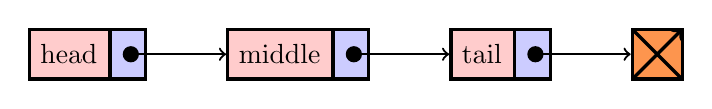
\begin{tikzpicture}[list/.style={
				very thick, rectangle split,
				rectangle split parts=2, draw,
				rectangle split horizontal, minimum size=18pt,
				inner sep=4pt, text=black,
				rectangle split part fill={red!20, blue!20}
			},
			->, start chain, very thick,
			chain_arrow/.style={*->, thick}]
		\node[list,on chain] (A) {head};
		\node[list,on chain] (B) {middle};
		\node[list,on chain] (C) {tail};
		\node[squarecross]   (D) [right=of C] {};
		\draw[chain_arrow] let \p1 = (A.two), \p2 = (A.center) in (\x1,\y2) -- (B);
		\draw[chain_arrow] let \p1 = (B.two), \p2 = (B.center) in (\x1,\y2) -- (C);
		\draw[chain_arrow] let \p1 = (C.two), \p2 = (C.center) in (\x1,\y2) -- (D);
	\end{tikzpicture}
\end{center}


\section*{Goal}

We can create a \texttt{LinkedList} by chaining simple nodes together. 
But, in this case the list is not really usable.
We have to store the first element in a variable and the use loops to access any element we want.
We want to use the \texttt{LinkedList} the same way we use a \texttt{list} in Python.
The first step is the encapsulation of the functionality of a list in a class.
We will define methods in that class that will provide functionality similar to a normal \texttt{list}.

Take the python file provided and extend the class to include the functionalities that are missing.
You can take a loot at the slides provided to get some hints on how to achieve each of the features.
You can try to program them in whatever order you prefer, there is no need to follow the order shown on this document.

\textbf{The functions should have the names shown in this document.}

\newpage
\subsection*{Inserting elements}

\begin{enumerate}
	\item Inserting at the head:
\begin{lstlisting}
lst = LinkedList()
lst.add_head("a")
print(lst)
# Output: a -> None
lst.add_head("b")
print(lst)
# Output: b -> a -> None
lst.add_head("c")
print(lst)
# Output: c -> b -> a -> None
\end{lstlisting}
	\item Inserting at the tail:
\begin{lstlisting}
lst = LinkedList()
lst.add_tail("a")
print(lst)
# Output: a -> None
lst.add_tail("b")
print(lst)
# Output: a -> b -> None
lst.add_tail("c")
print(lst)
# Output: a -> b -> c -> None
\end{lstlisting}
	\item Inserting anywhere by using an index, remember that indexes start at 0. The new element will be inserted after the given index:
\begin{lstlisting}
print(lst)
# Output: a -> b -> c -> None
lst.add_after(1, "d")
print(lst)
# Output: a -> b -> d -> c -> None
lst.add_after(1, "e")
print(lst)
# Output: a -> b -> e -> d -> c -> None
\end{lstlisting}
\end{enumerate}

\newpage

\subsection*{Removing elements}

\begin{enumerate}
	\item Remove the head:
\begin{lstlisting}
print(lst)
# Output: a -> b -> c -> None
lst.remove_head()
print(lst)
# Output: b -> c -> None
lst.remove_head()
print(lst)
# Output: c -> None
\end{lstlisting}
	\item Removing the tail:
\begin{lstlisting}
print(lst)
# Output: a -> b -> c -> None
lst.remove_tail()
print(lst)
# Output: a -> b -> None
lst.remove_tail()
print(lst)
# Output: a -> None
\end{lstlisting}
	\item Removing at an index:
\begin{lstlisting}
print(lst)
# Output: a -> b -> c -> e -> d -> None
lst.remove_index(2)
print(lst)
# Output: a -> b -> e -> d -> None
lst.remove_index(0)
print(lst)
# Output: b -> e -> d -> None
\end{lstlisting}
	\item Removing a given element:
\begin{lstlisting}
print(lst)
# Output: a -> b -> c -> e -> d -> None
lst.remove("b")
print(lst)
# Output: a -> c -> e -> d -> None
lst.remove("e")
print(lst)
# Output: a -> c -> d -> None
\end{lstlisting}
\end{enumerate}

\newpage

\subsection*{Other functionalities}

\begin{enumerate}
	\item Pretty print a the list in the console when using \lstinline|print(lst)|
	\item Get the size of the list:
\begin{lstlisting}
print(lst)
# Output: a -> b -> c -> e -> d -> None
print(lst.size())
# Output: 5
print(len(lst))
# Output: 5
\end{lstlisting}
	\item Check if an element exists in a list:
\begin{lstlisting}
print(lst)
# Output: a -> b -> c -> e -> d -> None
print(lst.contains("a"))
# Output: True
print(lst.contains("z"))
# Output: False
print("c" in lst)
# Output: True
print("x" in lst)
# Output: False
\end{lstlisting}
	\item Obtain an element at an index:
\begin{lstlisting}
print(lst)
# Output: a -> b -> c -> e -> d -> None
print(lst.get(1))
# Output: b
print(lst[2])
# Output: c
\end{lstlisting}
	\item Modify an element at an index:
\begin{lstlisting}
print(lst)
# Output: a -> b -> c -> e -> d -> None
lst.set(1, "z")
print(lst)
# Output: a -> z -> c -> d -> e -> None
lst[2] = "x"
print(lst)
# Output: a -> z -> x -> d -> e -> None
\end{lstlisting}
\end{enumerate}

\section*{Evaluating the Performance}
Not all list structures behave equally. Some may be more efficient in one operation, some on other and some might try to find a balance. We are going to compare the performance of the \lstinline|list| structure in Python, with our own \lstinline|LinkedList| and an implementation of a linked list that is provided by the \lstinline|collections| module, the \lstinline|deque|. In order to see the which operation has better performance we can simply use the time a computer needs to execute it.

\begin{attachedlisting}[time]
import time

start = time.perf_counter_ns()
x = (12 ** 124) ** 0.5
end = time.perf_counter_ns()

print(f"Time: {(end-start)/1e9:.10f} seconds")
\end{attachedlisting}

Have a look at the code, how much time does it need to perform the calculation? Run the code several times, is the time always the same or does it vary? What happens if we remove the code on line 4? Does it need some time to simply execute the statements to get the time in nanoseconds? Will it affect our measurements?

We can solve most of these problems by simply executing the same piece of code several times. By executing the same piece of code, let's say 1000 times, we reduce the effect of variations and time lost getting the counters.

\begin{attachedlisting}[time]
import time

start = time.perf_counter_ns()
for _ in range(1000):
    x = (12 ** 124) ** 0.5
end = time.perf_counter_ns()

print(f"Time: {(end-start)/1e9:.10f} seconds")
\end{attachedlisting}

Execute this several times, does the time still vary? Maybe instead of executing it 1000 times increase the value to 1000000. What happens? In order to get more consistent data we need to execute the code quite a few times.

Use the same structure to get the time a \lstinline|list|, \lstinline|LinkedList| and a \lstinline|deque| needs for the following operations, and fill the table with the time it requires for the amount of operations. For the first set of operations we will start with an empty list and add $n$ elements on a loop. For the get operations we need some data on the lists, so we can simply add a few dummy data points to the lists and then try to get them.

\newpage
Number of iterations: \rule{3cm}{0.15mm}\\

\begin{table}[h!bt]
\renewcommand{\arraystretch}{1.4}
\centering
\begin{tabular}{m{0.3\textwidth}m{0.2\textwidth}m{0.2\textwidth}m{0.2\textwidth}}
\toprule
Operation & \lstinline|list| & \lstinline|LinkedList| & \lstinline|deque| \\
\midrule
Insert at the head & & &\\
Insert at the tail & & &\\
Insert at index & & &\\
\midrule
Get head element & & &\\
Get tail element & & &\\
Get at index & & &\\
\bottomrule
\end{tabular}
\end{table}

\FloatBarrier

\newpage

\section*{Other improvements to a list}

\begin{enumerate}
	\item We have created a list where we can insert an element at any position we want. Now we want to have a list that is sorted. Create a \texttt{SortedLinkedList} class where we only have a method that allows the insertion of elements \texttt{SortedLinkedList.add(data)}. The method will insert the element at the correct position so that all the items in the list before the element will be smaller, and all the items after will be larger. Use the operands $<, >, <=, >=$ to compare the items in the list to the element to be inserted and find the position where it has to be added.
	\item We have created a list where each node only references to the next one. This creates a list where adding or removing the head of the list is really simple, and very efficient. We can extend this functionality by creating a \texttt{DoublyLinkedList}, in this case each node will not only point to the next element in the list, it will also contain the reference to the previous node in the list. In this case the class will not only hold a reference to the head, but also to the tail of the list. Effectively creating a structure with two lists going in opposite directions. Using this operation in the tail is as efficient as the operation at the head.
    \begin{figure}[h!bt]
	\begin{center}
	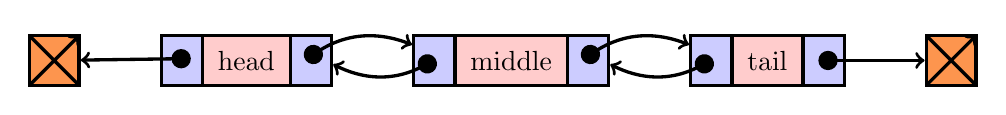
\begin{tikzpicture}[
		list/.style={
			very thick, rectangle split,
			rectangle split parts=3, draw,
			rectangle split horizontal, minimum size=18pt,
			inner sep=5pt, text=black,
			rectangle split part fill={blue!20, red!20, blue!20}
		},
		->, start chain, very thick
		]
		
		\node[list,on chain] (A) {\nodepart{second} head};
		\node[list,on chain] (B) {\nodepart{second} middle};
		\node[list,on chain] (C) {\nodepart{second} tail};
		
		\node[squarecross]   (D) [right=of C] {};
		\node[squarecross]   (E) [left= of A] {};
		
		\path[*->] let \p1 = (A.three), \p2 = (A.center) in (\x1,\y2) edge [bend left] ($(B.west)+(0,0.2)$);
		\path[*->] let \p1 = (B.three), \p2 = (B.center) in (\x1,\y2) edge [bend left] ($(C.west)+(0,0.2)$);
		\draw[*->] let \p1 = (C.three), \p2 = (C.center) in (\x1,\y2) -- (D);
		
		\draw[*->] ($(A.one)+(0.2,0.1)$) -- (E);
		\path[*->] ($(B.one)+(0.1,0.1)$) edge [bend left] ($(A.east)+(0,-0.05)$);
		\path[*->] ($(C.one)+(0.1,0.1)$) edge [bend left] ($(B.east)+(0,-0.05)$);
	\end{tikzpicture}
	\end{center}
    \end{figure}
\end{enumerate}

\end{document}